%%%%%%%%%%%%%%%%%%%%%%%%%%%%%%%%%%%%%%%%%
% CCaN Notes Exam
%
% Author: Tom Lonergan
%
%%%%%%%%%%%%%%%%%%%%%%%%%%%%%%%%%%%%%%%%%

%----------------------------------------------------------------------------------------
%	PACKAGES AND OTHER DOCUMENT CONFIGURATIONS
%----------------------------------------------------------------------------------------

\documentclass[fontsize=8pt]{scrartcl} % 8pt font size
\usepackage{amsmath}
\usepackage{amssymb}
\usepackage{amsthm}
\usepackage{multicol} % Required for multicolumn layout
\usepackage{color} % Required for color customization
\usepackage{arev}
\usepackage{graphicx}

\usepackage[a4paper, margin=25pt, landscape]{geometry} % Page margins and orientation

\usepackage[ % This block contains information used to annotate the PDF
colorlinks=false, 
pdftitle={CCaN Notes}, 
pdfauthor={Tom Lonergan}, 
pdfsubject={CCaN Notes}, 
]{hyperref}

\setlength{\parindent}{0pt} % Stop paragraph indentation
\pagenumbering{arabic} % Page numbering

%----------------------------------------------------------------------------------------

\begin{document}
\newtheorem*{definition}{Definition}
\newtheorem*{theorem}{Theorem}
\newtheorem*{corollary}{Corollary}

\begin{multicols*}{4}
	% Put your sections here...
	\section{Network overview}
\subsection{Access networks}
\textbf{Digital subscriber line (DSL)} uses existing telephone lines to transmit data at high frequencies, and voice at low frequencies. These two frequency ranges are separated using a DSL access multiplexer (DSLAM), with the voice frequencies going to the telephone network while the data goes to the internet. \\
\textbf{Cable} based access uses frequency division multiplexing (FDM) to allow many channels to transmit simultaneously by assigning each a frequency band. It can use TV lines, or dedicated internet lines. Shared wireless access networks connect end systems to routers via an access point or base station.\\
\textbf{Wireless local area network} (WLAN) typically connect in or around a building (~100ft range) with an up to 10 Gbps transmission rate. A wide area cellular access network is provided by a mobile service provider, with ranges in the 10s of kilometres and lower transmission rates (~100 Mbps for 4G, 1 Gbps for 5G). An enterprise network consists of a mix of wired and wireless access points.
\subsection{Physical media}
\textbf{Twisted pair} - a pair of insulated copper wires twisted together, which reduces electromagnetic interference. Cat5 and Cat6 cables use a number of twisted pairs, reaching 100 Mbps-1 Gbps and 10 Gbps speeds respectively.\\
\textbf{Coaxial cables} consist of an central copper wire, a layer of insulation, another layer of copper, and an outer sheath. This allows data to be bidirectionally transmitted, one way on each layer. Broadband cables are coax, with multiple frequency channels on each cable and can reach a speed of 100 Mbps per channel.\\
A \textbf{fibreoptic cable} contains a glass fibre carrying light pulses, with each pulse being a bit. They are extremely high bandwidth, with transmission rates up in the 10-100+ Gbps range, have a low error rate as they are immune to EM interference, but are expensive and inflexible.\\
\textbf{Wireless radio} - instead of using a cable, radio/microwaves are used to carry signals, which propagate across the environment. This removes the need to physically connect devices to the network, but comes at the cost of variable signal strengths, interference, and obstruction by non-radio-transparent objects. Types include: terrestrial microwave (up to 45 Mbps), wireless LAN (up to 1 Gbps), wide area (up to ~1 Gbps), and satellite (up to 45 Mbps, has either high latency for geosynchronous orbits or higher cost/complexity for low-earth-orbit satellites).
\subsection{Internet structure} The internet is assembled from a collection of ISPs of different scales:\\
A small number of large networks: \textbf{Tier-1} commercial ISPs (e.g. BT, Virgin Media, Sprint, AT\&T) which provide national and international coverage, and \textbf{content provider networks (CDNs)} (e.g. Google, Facebook) - private networks for connecting data centres to the internet, bypassing tier-1 and regional ISPs.\\
A large number of small networks: various lower tier ISPs, which resell access to some tier 1 ISP hardware or using their own regional networks. ISPs connect to each other at \textbf{IXPs (internet exchange points)}
\subsection{Delays}
\textbf{Processing delay}\\
When a packet arrives at a node, the header is examined and used to determine where the packet should be directed - this takes some time and is **processing delay**. Processing delays in modern high-speed routers are usually microseconds or less.\\
\textbf{Queuing delay}\\
After a packet is processed, it is added to queue to wait for its transmission link to become available. This is dependent on how many packets have arrived before it that are still waiting to be transmitted, if no packets have arrived recently then it will be close to 0, but if traffic is heavy then there may be a long delay. In practice, queuing delays are between microseconds and milliseconds.\\
\textbf{Transmission delay}\\
A link between routers will have a transmission rate in ($R$ bits per second). If a packet is of size $L$ bits, then it will take $L/R$ seconds to transmit one full packet. Transmission delays tend to be between microseconds and milliseconds in practice.\\
\textbf{Propagation delay}\\
Once a bit is pushed into a link, it must propagate down it to the next router. This is governed by the propagation speed (the speed that the signal can move within the link's medium, e.g. speed of light (~$3*10^8\text{ m/s}$) in fibre lines or the speed of electricity (~$2*10^8\text{ m/s}$) in copper). Propagation delay can be milliseconds in large networks, or nearly negligible in local ones.\\
\textbf{Overall delay}\\
If we let $d_{proc}$, $d_{queue}$, $d_{trans}$, $d_{prop}$ be the processing, queuing, transmission, and propagation delays respectively, then the total nodal delay
$$d_{nodal}=d_{proc}+d_{queue}+d_{trans}+d_{prop}$$
\textbf{Queuing delay in more detail}\\
Queuing delay is the most complex part of nodal delay, as it varies packet by packet. This means that we can't discuss absolute values but instead statistical measures of mean/median delays and their distributions, or in probabilities.
If we have $R$ = transmission rate, $a$ = packets per second, and $L$ = packet size, then we can calculate the traffic intensity:
$$
	\text{Traffic intensity }=\frac{La}{R}
$$
If $\frac{La}{R}>1$ then the average rate of bits arriving at the queue exceeds the rate at which they can be transmitted, resulting in the queue increasing forever and the queuing delay approaching infinity.
In the case $\frac{La}{R}\leq1$ the nature of arriving traffic impacts the queuing delay. E.g. if one packet arrives exactly every $\frac{L}{R}$ seconds then each packet will arrive to an empty queue and the will be no queuing delay. If the packets arrive in periodic bursts, e.g. $N$ packets every $\frac{NL}{R}$ seconds, then the first packet will have no queuing delay, the second an $\frac{L}{R}$ second delay, third a $\frac{2L}{R}$ delay, and so on with the $n$th packet having a $\frac{(n-1)L}{R}$ delay.

	\section{Protocol layers}
\textbf{Application}: works with messages. Is where applications and their protocols exist. Examples include HTTP, SMTP, FTP, and DNS.\\
\textbf{Transport}: works with segments. Transports application layer messages between specific applications on different hosts. Examples include TCP and UDP.\\
\textbf{Network}: works with datagrams. Transports segments from one host to another. Examples include IP and ICMP.\\
\textbf{Link}: works with frames. Transports datagrams between neighbouring network elements. Examples include Ethernet and WiFi.\\
\textbf{Physical}: works with bits. The physical medium connecting neighbouring network elements. Examples include copper cable, fibre optics, and radio waves.

\subsection{Application layer}
An application is identified by a 32 bit \textbf{IP address} and 16-bit \textbf{port number}. The IP address identifies the host, and the port number identifies the application on that host.

\subsubsection{The Web and HTTP}
\textbf{HTTP} is a stateless protocol which determines how web clients (such as browsers) interact with web servers. HTTP uses TCP, and either establishes one persistent session across many requests, which removes the expensive setup time for each request, or establishes a new session for each request, which prevents the client and server from needing to store information about a session that is not currently in use. When non-persistent sessions are used, each request takes approximately $2\cdot\text{round trip time}+\text{file transmission time}$, while with persistent sessions once a connection is established, each request takes approximately $\text{round trip time}+\text{file transmission time}$.\\
An \textbf{HTTP request} has this format:\\
\begin{verbatim}
GET /somedir/page.html HTTP/1.1
Host: www.someschool.edu
Connection: close
User-agent: Mozilla/5.0
Accept-language: fr
\end{verbatim}
Common request methods are: \textbf{GET} (request an object from the server), \textbf{POST} (send some data and the server should reply with a response object), \textbf{HEAD} (request an object, but the server only responds with the HTTP header, used for debugging), \textbf{PUT} (upload an object), \textbf{DELETE} (delete an object from the server). \textbf{GET} can also send data to the server, by appending queries to the URL, e.g. \verb|somesite.com/search?search=a+search+string|.\\
An \textbf{HTTP response} has this format:\\
\begin{verbatim}
HTTP/1.1 200 OK
Connection: close
Date: Tue, 18 Aug 2015 15:44:04 GMT
Server: Apache/2.2.3 (CentOS)
Last-Modified: Tue, 18 Aug 2015 15:11:03 GMT
Content-Length: 6821
Content-Type: text/html
data goes here
\end{verbatim}
Common response codes are: \textbf{200 OK} (request succeeded), \textbf{301 Moved Permanently} (requested object has been moved, the client will automatically request the new URL), \textbf{400 Bad Request} (message not understood by server), \textbf{404 Not Found} (requested document not found), \textbf{505 HTTP Version Not Supported} (server does not support the HTTP protocol version used in the request).\\
Sessions can be tracked using \textbf{cookies} by setting the \textbf{Set-Cookie} header in the response, and the client will send the cookie back in the request. Cookies can be used to store session information, user preferences, and shopping cart contents, or they can be IDs that are used to index a cookie database on the server.\\
\textbf{HTTP/2} is a new version of HTTP that is binary instead of textual, fully multiplexed, uses one connection for parallelism, uses header compression, and allows servers to push responses proactively into client caches.
\textbf{Web caches} satisfy HTTP requests on behalf of a server. A browser must be configured to request from a cache, and then if the page is already in the cache it can respond faster than the server could have. Web caches use conditional GETs to check if the page has been updated since the last time it was cached, by setting the \verb|If-Modified-Since| header line.\\

\subsubsection{Email and SMTP}
Email systems consist of user agents, mail servers, and the simple mail transfer protocol (STMP). When an email is sent, the user agent sends the email to the user's mail server, which then sends the email to the recipient's mail server, which then stores the email until the recipient's user agent requests it. STMP uses TCP with persistent connections, and pushes the email to the recipient's mail server, unlike HTTP which pulls objects from a server. An email header looks like this:
\begin{verbatim}
From: alice@aServer.com
To: bob@anotherServer.com
Subject: Hello
\end{verbatim}
\textbf{POP3} is a protocol used by the recipient's mail client to retrieve the email from the server. A user logs in with \verb|user <username>| and \verb|pass <password>|, then can list emails with \verb|list|, retrieve an email with \verb|retr|, and delete an email with \verb|dele|. Once the user has finished, all their actions are applied at the same time with \verb|quit|.\\
\textbf{IMAP} is a protocol used by the recipient's mail client to retrieve the email from the server. It is more powerful than POP3, as it allows the user to create, delete, and rename mailboxes, and allows the user to search for emails.\\
Today, most email clients are sent using a web browser, so emails are requested from servers using HTTP.

\subsubsection{DNS}
The \textbf{Domain Name System} is responsible for translating application layer hostnames to network layer IP addresses. It is a distributed database implemented in a hierarchy of DNS servers. When a request is made, the DNS client calls a local DNS server, which then calls a root DNS server, which then calls a top-level domain DNS server, which then calls an authoritative DNS server. The authoritative DNS server then sends the IP address back to the client. The local server will cache the IP address of the response, but will also cache the addresses of the various servers, meaning that the root servers are very rarely contacted. DNS resolution uses both recursive requests (the client asks the server to resolve the request) and iterative requests (the client asks the server to tell it the next server to contact). A hostname may map to many IP addresses, in which case the server responds with them in a random order. As the client usually picks the first one, this acts as a simple load balancing system.\\
A DNS request has this format:
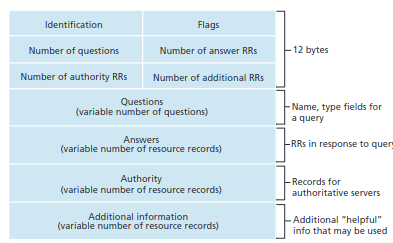
\includegraphics[width=\linewidth]{../images/w3n7dnsMessage.png}\\
And a record has the format \verb|<name, value, type, ttl>|. The \textbf{type} states what the record is, \verb|A| means \verb|name| is a hostname and \verb|value| is the corresponding IP address, \verb|NS| means \verb|name| is a domain and \verb|value| is the server knows the next step in resolving that domain, \verb|CNAME| means \verb|name| is an alias for \verb|value|, \verb|MX| means \verb|name| is a domain and \verb|value| is the mail server for that domain. The \textbf{ttl} is the time the record can be cached for.\\

\subsubsection{P2P and BitTorrent}
\textbf{Peer-to-peer} applications communicate directly with other peers without requiring a central server. P2P applications are used for file distribution, streaming, and telephony, as they are well suited to sharing large files.\\
If we have a system with $N$ hosts wishing to download an $F$ bit file, peer[$i$] having an upload rate of $u_i$ and a download rate of $d_i$, along with a server with an upload rate of $u_s$, then for a client server architecture the time for all clients to download the file is bounded by
$$
	D_{CS}\ge\max\left\{\frac{NF}{u_s},\frac{F}{d_{\min}}\right\}
$$
In a P2P system, each peer who gets a part of the file can distribute it onwards, and the download time is bounded by
$$
	D_{P2P}\ge\max\left\{\frac{F}{u_s},\frac{F}{d_{\min}},\frac{NF}{u_s+\sum^N_{i=1}u_i}\right\}
$$
$D_{P2P}$ equals that only when the server sends bits one at a time to each client.\\
\textbf{BitTorrent} is a popular P2P file distribution protocol. A file is broken into chunks, typically 256 KB each, and all peers for a file form a torrent. Each torrent has a tracker, which keeps a list of all active peers. When a new peer (we'll call Alice) joins a torrent, it contacts the tracker, which selects a random subset of peers and sends their IPs to Alice who attempts to open concurrent TCP connections with all the IPs it received. Each successful connection is counted as a "neighbouring peer", and over time some of those peers will leave while others join and establish connections, leading to Alice's neighbouring peers fluctuating over time. Every neighbour will have a different subset of chunks of the file, so Alice will periodically request a list of the chunks each of its neighbours has. Alice then determines which chunks are held by fewest of her neighbours and requests them first (rarest-first), this means that each chunk of a file should end up roughly equally distributed.\\
Alice will also receive requests for chunks for each of her neighbours, and she selects the four that are sending her the highest rate of bits, and reciprocates by sending them their requested chunks - these neighbours are known as **unchoked**. She recalculates the top four every 10 seconds. Every 30 seconds, she also selects one random neighbour (in this case Bob) and sends it chunks - this neighbour is **optimistically unchoked**. If Alice makes it into Bob's top four uploaders and he will reciprocate, and may also make it into Alice's top four. This means that peers will gradually match up with other peers that are capable of uploading at comparable rates, and that a new peer will get chunks that it can trade with its neighbours. All other neighbouring peers receive nothing from Alice, and are **choked**.

\subsection{Transport layer}

\subsubsection{TCP}
\textbf{Transmission Control Protocol} provides a delivery service that guarantees that a byte stream sent using it will arrive in order with no duplicate packets. It is a \textbf{connection oriented service}, meaning that the client and server exchange transport layer level control information before the application layer messages start to flow.


\subsection{Network layer}
\subsection{Link layer}

\end{multicols*}

\end{document}
